\documentclass[aps,rmp,preprint,superscriptaddress,10pt,onecolumn]{article}
\usepackage[utf8x]{inputenc}
\usepackage{amsmath,amsthm,amsfonts,amssymb,amscd}
\usepackage{graphicx}
\usepackage{wrapfig}
\usepackage{enumerate}
\usepackage{color}
\usepackage[final]{hyperref}
\usepackage{fontspec}
%\usepackage{natbib}
%\bibliographystyle{plainnat}


\setmainfont{Times New Roman}
\usepackage{unicode-math}
\setmathfont{XITS Math}


%\setlength{\parindent}{20pt}
\def\thesubsectiondis{\unskip\arabic{subsection}}
 
\begin{document}

\title{Data summary:\\\textit{Growth: From Microorganisms to Megacities}, Vaclav Smil (2009)}
\author{Liam P. Shaw}
\date{\today}


\maketitle

\section*{Summary}

\noindent This document contains graphs fitted from a variety of datasets in \textit{Growth} (Smil, 2009). 

\par

\section*{Chapter 1}

\begin{figure}[h]
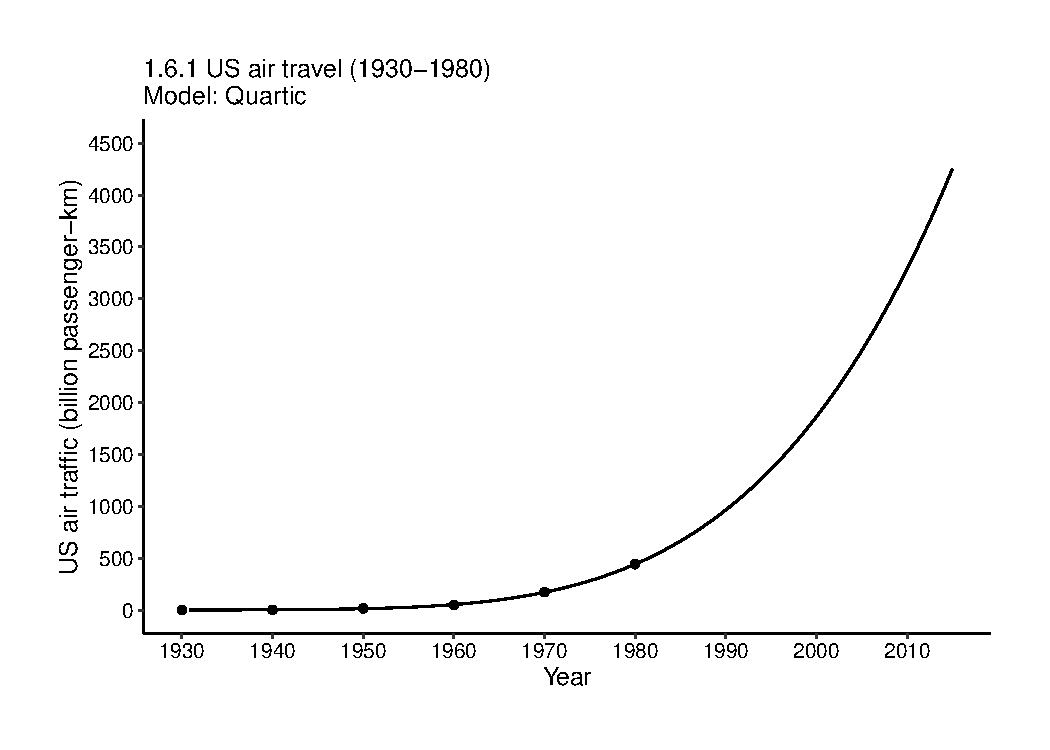
\includegraphics[width=8cm]{output/figs-ggplot/1.6.1.pdf}
\caption{}
\end{figure}





\section{Data availability}

\noindent Code and data to reproduce analysis are available at \url{https://github.com/liampshaw/Smil-Growth-2009}. 

\bibliography{cite}{}

\end{document}
